% Initial and revised submissions should be 12 point; this will be removed in the final version.
\documentclass[12pt]{TD-CJS}

% Initial and revised submissions should also be double spaced.  This command will be removed in the final version.
\renewcommand{\baselinestretch}{2}

\usepackage{latexsym}
\usepackage{amsmath}
\usepackage{amsfonts}
\usepackage{amssymb}
\usepackage{psfrag}
\usepackage{graphicx}
\newcommand{\argmin}{\operatornamewithlimits{argmin}}
\usepackage{float}
\usepackage[caption = false]{subfig}
% \usepackage[authoryear,round]{natbib}
% \usepackage{Cjsref}
\usepackage{xcolor}

\begin{document}
\firstpage{1}
\lastpage{25}
\jvol{xx}
\issue{yy}
\jyear{2019}
\jid{CJS}
\aid{2019}
% The running head contains the author names
\rhauthor{BlindedA and BlindedB}
\copyrightline{Statistical Society of Canada}
\Frenchcopyrightline{Soci\'et\'e statistique du Canada}
% History: received and accepted dates
\received{\rec{9}{July}{2019}}
\accepted{\acc{8}{July}{2010}}

% User-defined commands go here
\renewcommand{\eqref}[1]{(\ref{#1})}
% \newcommand{\mb}[1]{\mathbf{#1}}
% \newcommand{\mbb}[1]{\mathbb{#1}}
% \newcommand{\mt}[1]{\mathrm{#1}}
% \newcommand{\rv}{random variable}

% Title, authors, affiliations
\title[]{Optimal design under complete class with ancillary functions}%\query{Q1}
\author{BlindedA\authorref{1}\thanksref{*}}
\author{BlindedB\authorref{2}}
\affiliation[1]{Author affiliations will go here in the accepted manuscript, 
but do NOT include them in your initial submission because it must be anonymous.}
\affiliation[2]{Second Affiliation}

% Abstract, keywords, and classification codes
\startabstract{%
\keywords{
\KWDtitle{Key words and phrases}
Ancillary functions \sep complete class\sep minimally-supported design\sep nonlinear models\sep  Tchebycheff system .
% MSC 2010 subject classification codes
\KWDtitle{MSC 2010}  Primary 62K05}
\begin{abstract}
\abstractsection{}
\abstractsection{Abstract}
Nonlinear models are challenging in optimal designs due to the complexity and lack of canonical forms. The complete class strategy provided a unified framework for studying optimal designs for nonlinear models. However, due to the assumptions of the current strategy, many models are not applicable under this framework. In this paper, we propose a tool called ancillary functions as an extension to the complete class strategy. We also provide results on minimally supported designs with proper conditions. This tool is demonstrated with two-parameter dose-response models including the Beta-Poisson model, complementary log-log model, and skewed logit model. The results of this paper add to the previous complete class framework and make the minimally supported design available for more nonlinear models that were previously not feasible.  

% Insert your abstract here; it should
% typically be up to ten lines long. Avoid symbols as much as possible. Formulas
% are strongly discouraged, and citations should be avoided. 
% The title and the abstract should be concise and descriptive;
% list the key words in alphabetical order.  The MSC 2010 subject classification codes can be found here:
% http://www.ams.org/mathscinet/msc/pdfs/classifications2010.pdf.
\abscopyright
\fabstractsection{}
% \fabstractsection{R\'{e}sum\'{e}}
% Ins\'{e}rer votre r\'{e}sum\'{e}
% ici. We will supply a French abstract for those authors who
% can't prepare it themselves.\Frenchabscopyright
\end{abstract}}
\makechaptertitle

% Email address for corresponding author
\correspondingauthor[*]{\\\email{Insert your email address here only after your paper has been accepted}}

\section{INTRODUCTION}
Scientific studies rely on controlled experiments to investigate causal effects. While more experimental resources usually lead to more information gain, seeking the trade-off between the two aspects matters in reality and drives the demand of ``good" experimental designs. Optimal designs as a class of experimental designs address and formulate this balance: the ``information" is defined through different statistical criteria; the ``cost" is measured by the total number of experimental runs. 





% An approximate design $\xi$ is comprised of the support points $x_i$'s and the corresponding weights $w_i$'s. An optimal design seeks the best choice of $\xi = \{(x_i,w_i), i=1,\ldots,n\}$ that maximizes the optimality criterion given a model. 

There is extensive research on optimal designs for linear models. However, for nonlinear models, the problem is remarkably different. The complications of nonlinear models lie in two aspects. First, the information matrix of a nonlinear model depends on the unknown model parameters $\theta$: the choice of an optimal design $\xi$ relies on presumed values of $\theta$, leading to locally optimal designs. 
Second, since nonlinear models do not have a canonical form, the complexity and variety make the derivation and the numerical search a challenge. The locally optimal designs can be resolved with sequential designs where we can adaptively update the estimate of $\theta$.
On the second aspect, most available results are based on the geometric approach by Elfving (1952) or equivalence theorem by Kiefer \& Wolfowitz (1960) that deal with certain types of nonlinear models for specific optimality criteria. These results provide case-by-case solutions only and lack overarching results.




Some recent advances extended possibilities in identifying optimal designs for nonlinear models. Yang \& Stufken (2009, 2012), Yang (2010), Dette \& Melas (2011), and Dette, Melas, \& Shpilev (2013) provided a unified strategy to identify the optimal designs through a complete class. This strategy characterizes a complete class of designs with the number of support points $n$ such that, for any design $\xi$, there exists a design $\xi^*$ in the complete class that dominates $\xi$ in terms of Loewner ordering. Although this strategy does not provide a specific optimal design, we could focus on this complete class of designs for further numerical search or mathematical derivation of optimal design $\xi^*$. Also, the generality of Loewner ordering as the optimality criterion broadens the application scenarios where any information-based optimality criteria may be used.

% enables us to apply any information-based optimality criteria and thus is highly flexible for various application scenarios.

While the complete class strategy has made substantial progress, certain models are not yet applicable due to the assumptions in the current results. In this paper, we propose a new tool called Ancillary Functions to extend the results of Yang (2010) and Yang \& Stufken (2009, 2012) to many new nonlinear models. While involving ancillary functions seems increasing the number of support points needed, we show in our results that under certain conditions, we can remove the extra points and obtain a minimally supported locally optimal design. We also demonstrate our approach with the Beta-Poisson model, complementary log-log model, and skewed-logit model. With the Beta-Poisson model and complementary log-log model, we obtained the complete class of minimally supported optimal designs. These minimally supported design classes were not feasible through the previous approaches.  
 
In this paper, we discuss the model setup in Section \ref{2} and introduce the current methodology and limitations in Section \ref{metho}. We present our main results in Section \ref{main} and further discussions in Section \ref{dis}. 

\section{Model and Approximate Design}\label{2}
Consider a nonlinear regression model $ E(y) = \eta(x,\theta)$, where a response variable $y$ depends on a single regression variable $x$. Assume $y$'s are independent and follow a distribution from the exponential family with mean  $\eta(x,\theta)$. In Design of Experiment, the variable $x$ represents a design point. For some $N>0$, the collection of design points and the weights $\xi = \{(x_i,w_i), i=1, \ldots,
N\}$, $\sum_{i=1}^Nw_i = 1$, $w_i> 0$ is called an approximate design. In many cases, instead of $x_i$, it is more convenient to use $z_i$ as a monotonically continuous function of $x_i$. For what follows, we use $\xi = \{(z_i,w_i), i=1, \ldots,N\}$, $\sum_{i=1}^Nw_i = 1$ to denote the target design. 

The Fisher information matrix $M(\xi,\theta)$ of design $\xi$ and parameter $\theta$ can be written as 
% \begin{equation}\label{eq:1}
% M(\xi,\theta)  = P(\theta)(\sum_{i=1}^Nw_iC(\theta,z_i))P(\theta)^T
% \end{equation}where \begin{equation}\label{eq:2}
% C(\theta,z_i) = \left ( \begin{array}{cccc}
% \Psi_{11}(z_i) &&&\\
% \Psi_{21}(z_i) &\Psi_{22}(z_i)&&\\
% \vdots & \vdots &&\\
% \Psi_{p1}(z_i) &\Psi_{p2}(z_i)&\cdots&\Psi_{pp}(z_i)\\
% \end{array} \right).\end{equation}
\begin{equation}\label{eq:1}
M(\xi,\theta)  = P(\theta)(\sum_{i=1}^Nw_iC(\theta,z_i))P(\theta)^T
\end{equation}where \begin{equation}\label{eq:2}
C(\theta,z_i) = \left ( \begin{array}{c}
\Psi_{jl}(z_i)
\end{array} \right)_{p\times p}.\end{equation}
The matrix $P(\theta)$ is independent of $z_i$'s and $C(\theta,z)$ is symmetric. The functions $\Psi_{jl}(\theta,z), j,l=1,\ldots,p$ may depend on $\theta$, and as a result, so is $M(\xi,\theta)$. For the simplicity in notation, we drop the $\theta$ and use $\Psi_{jl}(z)$ and $M(\xi)$ instead for what follows. 

An optimal design $\tilde{\xi} = \{(\tilde{z}_i,\tilde{w}_i), i=1,\ldots,n\}$ minimizes a function of variance-covariance matrix of parameter of interest. Choice of the function needs to be statistically meaningful to evaluate the parameter estimation. 
% For example, D-optimality finds \begin{align*}
%     \tilde{\xi}&=\argmin_\xi det\left[\Sigma(\xi, \theta)\right]\\
%      & \approx \argmin_\xi det\left[(\frac{\partial \theta}{\partial \theta})M^{-1}(\xi)(\frac{\partial \theta}{\partial \theta})^T\right],
% \end{align*}
%  which measures the volume of the confidence ellipse for $\theta$.

In the mathematical derivation and numerical search of $\tilde{\xi} = \{(\tilde{z}_i,\tilde{w}_i), i=1,\ldots,n\}$ from the design space, a critical step is to determine the number of support points $n$.  The complete class approach identifies a complete class of designs with $n$ support points that satisfies the following: For any design $\xi=\{(z_i,w_i), i=1,\ldots,N\}$ with $N$ support points, there exists a design $\tilde{\xi} = \{(\tilde{z_i},\tilde{w_i}), i=1,\ldots,n\}$ with $n$ support points in the complete class that dominates $\xi$ in terms of Loewner ordering as follows
\begin{equation}\label{l-ordering}
    M(\xi)\le M(\tilde{\xi}).
\end{equation} Here the inequality means $M(\tilde{\xi})-M(\xi)$ is a non-negative definite matrix. As a result, the complete class is guaranteed to contain the optimal design in terms of Loewner ordering, which defines a general comparison between two information matrices. Notice that, $M(\tilde{\xi})-M(\xi)$ is non-negative definite matrix is equivalent to $C(\tilde{\xi})-C(\xi)$ is non-negative definite matrix. It is relatively easier to work on $C(\xi)$ instead of $M(\xi)$.
% In particular, optimality in Loewner ordering is sufficient to optimality in any traditional convex information-based criteria, including but not restricted to A-, D- and E-optimality. With this complete class, we can conduct a numerical search or mathematical derivation of optimal design $\tilde{\xi}$.
% With this complete class, we can conduct the numerical search or mathematical derivation of optimal design $\tilde{\xi}$ regardless of what information-based criteria are used.

% Loewner ordering in Equation \eqref{l-ordering} can be shown in various approaches.
There are various sufficient conditions for Loewner ordering in Equation \eqref{l-ordering}. Yang \& Stufken (2012) introduced a sufficient condition as follows. 

For some integer $p_1$, $1\le p_1<p$, partition $C(\theta,z_i)$ as \begin{equation}\label{def_block}
    C(\theta,z_i) = \left(\begin{array}{cc}
      C_{11}(z_i)   &  C_{21}^T(z_i) \\
        C_{21}(z_i)  & C_{22}(z_i) 
    \end{array}\right).
\end{equation} Here, $C_{22}(z_i)$ is the lower $p_1\times p_1$ principal sub-matrix of $C(\theta,z_i)$, that is 
\begin{equation}\label{def_c22}
    C_{22}(z_i) = \left( \begin{array}{ccc}
      \Psi_{p-p_1+1, p-p_1+1}(z_i)   & \cdots & \Psi_{p-p_1+1, p}(z_i) \\
      \vdots & \ddots & \vdots\\
        \Psi_{p, p-p_1+1}(z_i)   &\cdots  & \Psi_{p, p}(z_i)  
    \end{array}\right).
\end{equation} Hence, Equation \eqref{l-ordering} follows if it holds that 
\begin{align}\label{eq: strategy1}
    \sum_{i=1}^Nw_iC_{11}(z_i) &= \sum_{i=1}^n \tilde{w}_iC_{11}(\tilde{z}_i)\\
    \sum_{i=1}^Nw_iC_{12}(z_i) &= \sum_{i=1}^n \tilde{w}_iC_{12}(\tilde{z}_i)
\end{align} and 
\begin{equation}\label{eq: strategy2}
    \sum_{i=1}^Nw_iC_{22}(z_i) \le \sum_{i=1}^n \tilde{w}_iC_{22}(\tilde{z}_i)
\end{equation}


Instead of Equation \eqref{l-ordering}, its sufficient condition in Equations \eqref{eq: strategy1}-\eqref{eq: strategy2} can be used to find the complete class of designs with $n$ support points. This complete class contains a design that is at least as good as the optimal design in Loewner ordering. \\

{\color{blue} Choice of $p_1$ in \eqref{def_block} is a relatively more complicated problem, as it depends on the nonlinear model of interest. An examples of the choice was for exponential regression model \[Y_i = a_1e^{-\lambda_1x_i} + a_2e^{-\lambda_2x_i} + \epsilon_i.\] discussed in Yang \& Stufken (2012).
In this scenario $p=4$ with 4 parameters - $\lambda_1, \lambda_2, a_1, a_2$, and  $p_1$ was chosen to be 2 based on the model properties. We demonstrate in Section 4.3 - 4.5 of this paper with examples on how to choose $p_1$ as well.

}

\section{Methodology and limitations} \label{metho}
To identify the complete class of designs with $n$ support points, Yang \& Stufken (2012) and Dette \& Melas (2011) used Tchebycheff System (abbreviated ``T-system") as a bridge towards Equations \eqref{eq: strategy1} - \eqref{eq: strategy2}. The definition of a T-system is as follows.

\begin{theorem}{Definition 1}{}\label{deft}
    Let $u_0, \ldots, u_k$ denote continuous real-valued functions defined on a closed finite interval $[a,b]$, these functions form a \textbf{T-system} over $[a,b]$ provided  
\begin{equation}\label{eq: tdef2}
    U(u_0,\ldots,u_k, t_0,\ldots,t_k) = det\left ( \begin{array}{cccc}
u_0(t_0) &u_0(t_1) &\ldots &u_0(t_k) \\
u_1(t_0) &u_1(t_1) &\ldots &u_1(t_k) \\
\vdots & \vdots &&\vdots\\
u_n(t_0) &u_k(t_1) &\ldots &u_k(t_k) \\
\end{array}\right)
\end{equation}
     is strictly positive whenever $a\le t_0 <t_1< \ldots< t_k\le b$.
\end{theorem}
For simplicity, we use $U(t_0,\ldots,t_k)$ to denote the left-hand side of Equation~\eqref{eq: tdef2} for the following. 
Define a function sequence $\{\Psi_0(z),\Psi_1(z),\ldots, \Psi_k(z)^Q\}$ as follows: Partition $C(\theta,z)$ as in Equation \eqref{def_block} and Equation \eqref{def_c22} and let $\Psi_1(z),\ldots,\Psi_{k-1}(z)$ to be the maximum set of linearly independent non-constant terms in $C_{11}(z)$ and $C_{21}(z)$; Also define $\Psi^Q_{k}(z)$ as \[\Psi_k^Q(z) = Q^TC_{22}(z)Q\] where $Q$ is a nonzero vector of dimension $p_1\times 1$; Let $\Psi_0(z) = 1$ ( {\color{blue} see Section 4.3-4.5 for examples of these functions}). Yang \& Stufken (2012) showed that, given this function sequence  and considering the $\Psi_i$ as $u_i$ functions in the T-system, we can identify a complete class of designs with the number of support points if one of the two following conditions holds. % \begin{theorem}{Theorem 1}{}\label{2012a}
% For a regression model with a single regression variable $x$, suppose that the information matrix $M(z)$ can be written as in Equation \eqref{eq:1}-\eqref{eq:2} for $z\in[A,B]$. Partitioning $C(\theta,z)$ as in Equation \eqref{def_block} and Equation \eqref{def_c22} and let $\Psi_1(z),\ldots,\Psi_{k-1}(z)$ to be the maximum set of linearly independent non-constant terms in $C_{11}(z)$ and $C_{21}(z)$. $\Psi^Q_{k}(z)$ is defined as \[\Psi_k^Q(z) = Q^TC_{22}(z)Q\] where $Q$ is a nonzero vector of dimension $p_1\times 1$. Here $\Psi_0(z) = 1$.
% Suppose that either 
\begin{equation}
    \{\Psi_0(z),\Psi_1(z),\ldots, \Psi_{k-1}(z)\} \text{ and }  \{\Psi_0(z),\Psi_1(z),\ldots, \Psi_k(z)^Q\}
    \label{eq: 3.5}
\end{equation} form T-systems, or\begin{equation}\label{eq: 3.6}
    \{\Psi_0(z),\Psi_1(z),\ldots,\Psi_{k-1}(z)\} \text{ and }  \{\Psi_0(z),\Psi_1(z),\ldots, -\Psi_k(z)^Q\} 
\end{equation}
     form T-systems.
% Then the following results hold:
% \begin{enumerate}[(1)]
%     \item  For $k=2l-1$, $l\in \mathbb{Z}^+$, if Equation \eqref{eq: 3.5} holds, the designs with at most $l$ support points, including $B$, form a complete class
%     \item  For $k=2l-1$,  $l\in \mathbb{Z}^+$, if Equation \eqref{eq: 3.6} holds, the designs with at most $l$ support points, including $A$, form a complete class
%       \item  For $k=2l$, $l\in \mathbb{Z}^+$, if Equation \eqref{eq: 3.5} holds, the designs with at most $l+1$ support points, including both $A$ and $B$, form a complete class
%       \item  For $k=2l$,  $l\in \mathbb{Z}^+$,if Equation \eqref{eq: 3.6} holds, the designs with at most $l$ support points form a complete class
%     \end{enumerate}
% \end{theorem}
% Here the function sequence $\{\Psi_0(z)$, $\Psi_1(z)$, $\ldots$,$\Psi_{k-1}(z)$, $\Psi_k(z)^Q\}$ forming a T-system means that the determinant \[U(\Psi_0(z),\ldots,\Psi_k^Q(z), z_0,\ldots,z_k),\] denoted $U(z_0,\ldots,z_k)$, is strictly positive whenever $A\le z_0 <z_1< \ldots< z_k\le B$. 

This result directly leads to Equations \eqref{eq: strategy1}-\eqref{eq: strategy2} where $n$ indicates the number of support points. Therefore, at least one design in the complete class of designs is guaranteed to be optimal in terms of Loewner ordering. 

Since the sign of matrix determinant is invariant to certain row operations, and each function in the sequence represents one row, we can perform similar operations on the functions to ``alter" the T-system.  We could multiply each $\Psi_i()$ function by any function $g()$, $g(z_i)>0$ for all $z_i\in [A,B]$, $i=0,\ldots,k$ and $A\le z_0 <z_1< \ldots< z_k\le B$ with the sign of $U(z_0,\ldots,z_k)$ unchanged. We could also find $a^0_i,\ldots,a^k_i\in \mathbb{R}$ that form a new sequence of same length using linearly independent combinations of functions \[\{a^0_i\Psi_0(z)+\ldots+a^{k-1}_i\Psi_{k-1}(z)+a^k_i\Psi_k^Q(z) | i=0,\ldots,k\}\] such that the sign of $U(z_0,\ldots,z_k)$ is unchanged. However, since the order of functions in the sequence corresponds to the order of rows in the matrix, switching the order of neighboring functions would change the sign of $U(z_0,\ldots,z_k)$. As a result, we need to be cautious with the order of the functions in application. The three operations, when properly used, help form a simpler sequence in the T-system without changing the determinant and would be further discussed in Section~\ref{main}.


The result of Yang \& Stufken (2012) mentioned above connects the complete class with the T-system, but it is complicated to show a sequence of functions to be a T-System directly. To achieve that, Yang (2010) and Yang \& Stufken (2009, 2012) developed a tool to provide a sufficient condition for a sequence of functions to be a T-system. For $\{\Psi_0(z)$, $\Psi_1(z)$, $\ldots$,$\Psi_{k-1}(z)$, $\Psi_k(z)^Q\}$ defined as aforementioned, define functions $f_{l,t}, 1\le t \le k$, $t\le l \le k$ as
\begin{equation}
    \label{eq: ff}
f_{l,t}(z) = \left \{ \begin{array}{ll}
\Psi_l'(z), & \text{if } t=1,l=1,...,k-1\\
C'_{22}(z), & \text{if } t=1,l=k\\
(\frac{f_{l,t-1}(z)}{f_{t-1,t-1}(z)})', & \text{if } 2\le t\le k, t\le l \le k.
\end{array}\right.
\end{equation}

and   $F(z) = \prod_{l=1}^k f_{l,l}(z)$. 

Yang \& Stufken (2012) showed that $F(z)$ can be used to identify a complete class: $F(z)$ being positive definite is a sufficient condition of Equation \eqref{eq: 3.5}; $-F(z)$ being positive definite is a sufficient condition of Equation \eqref{eq: 3.6}. However, this sufficiency is based on three critical assumptions in definitions of $f_{l,t}(z)$ and $F(z)$.
\begin{enumerate}[(1)]
\item All functions $\Psi$ in the information matrix $C(\theta,z)$ are at least $k$th order differentiable on $(A,B)$.
\item For $1\le l\le k-1$, the functions $f_{l,l}(z)$ have no roots in $[A,B]$.
\item Either $F(z)$ or $-F(z)$ is positive definite for all $z\in [A,B]$.
\end{enumerate} 


 This strategy has been applied to many non-linear dose-response models such as logistic model, LINEXP model (Demidenko, 2006), and double-exponential regrowth model. But there are some models that are not applicable due to the assumptions. For example, a complementary log-log model has the following form. \[P(y=1|x) = 1-e^{-e^{z}}, z\in(-\infty,\infty)\] with which we could obtaib function sequence $\{1,g(z),$ $zg(z),z^2g(z)\}$, where \[g(z)=\frac{e^{2z}}{e^{e^z}-1}.\] 
 {\color{blue}The $f_{l,t}$ functions are then\[f_{11} = g'(z)\]
\[f_{2,1} = g(z)+zg'(z), f_{2,2} = 1+ (\frac{g(z)}{g'(z)})'\]
\[f_{3,1} = 2zg(z)+z^2g'(z), f_{3,2} = 2z+ (\frac{2zg(z)}{g'(z)})'\]
\[f_{3,3} = (\frac{ f_{3,2}}{ f_{2,2}})' =  (\frac{ 2z+ (\frac{2zg(z)}{g'(z)})'}{ 1+ (\frac{g(z)}{g'(z)})'})'  \]}
 With Mathematica, calculations shows that $f_{1,1}(z) = g'(z)$ has a root at $z=0.4660$, and $F(z)$ has a root at $z=0.0491$, which violates Assumptions (2) and (3). According to Yang \& Stufken (2012), we can only obtain the complete class for three disjoint intervals of z, $(-\infty, 0.0491)$, $(0.0491, 0.4660)$, and $(0.4660,\infty)$ separately, each with 2 support points. Yang \& Stufken (2009) introduced a method to combine designs for two intervals that are symmetric about zero and demonstrated with the 2-parameter logistic model. However, since there is no symmetry existing among the three intervals for the complementary log-log model, we cannot combine them and obtain a single unified design with the current approach.

 
\section{Main Results}\label{main}
The order and divergence rates of $\Psi_i(z)$'s play an essential role in the calculations of $f_{l,t}(z)$ and $F(z)$ and, in a way, determine the validity of the assumptions. A good ``tier" of $\Psi_i(z)$'s preserves the sign of $U(z_0,\ldots,z_k)$ and may be obtained by multiplying a positive function $g(z)$ to each function, forming linear combinations, or switching of terms in the sequence properly. LINEXP model and double-exponential model by Yang \& Stufken (2012) are successful examples. However, the good tier may not exist with the function sequence available, especially for nonlinear models like complementary log-log model which does not have an even link function. To address this issue, we propose a tool called \textit{Ancillary Functions}, with which we manually insert a few functions in the function sequence to form a good tier that satisfies the assumptions. 


\subsection{The Ancillary Functions} 
\begin{theorem}{Definition 2}{}\label{anci}
    For nonlinear model $E(y) = \eta(x,\theta)$, let \[S_1 = \{\Psi_0(z), \Psi_1(z), \ldots,\Psi_{k-1}(z) ,\Psi_k^Q(z)\}\] be functions defined in $C(\theta,z)$. Denote a set of functions \[ S_2 =\{\phi^*_1(z), \phi^*_2(z),\ldots, \phi^*_{k_1}(z)\}\] where $\phi^*_i(z)$, $i=1,\ldots,k_1$ are at least $(k+k_1)$-th order differentiable. Functions in $S_2$ are mutually linearly independent and independent of functions in $S_1$. We call $S_2$ as Ancillary Functions of $S_1$.
\end{theorem}

  Insert $\phi_i^*(z)$'s of $S_2$ to $S_1$ and apply modification or permutation as needed. Denote the new sequence as  \[S_3 = \{\tilde{\Psi}_0(z), \tilde{\Psi}_1(z), \ldots,\tilde{\Psi}_{k+k_1-1}(z), \tilde{\Psi}_{k+k_1}^Q(z)\},\]
  where $\tilde{\Psi}_{k+k_1}^Q(z) = \Psi_{k}^Q(z)$ is required after permutation. For a proper choice of $S_2$, working with $S_3$ instead of $S_1$ could form a better organized tier that satisfies the assumptions. The sign of $U(z_0,\ldots,z_k)$ with the new sequence $S_3$ will only change according to the order of functions in $S_1$ (before modification through multiplication or addition). The order or positions of the ancillary functions are irrelevant. The details of application are demonstrated in Section \ref{secbeta}-\ref{secskew}.


Rewrite Equation \eqref{eq: strategy1}-\eqref{eq: strategy2} using the $\Psi_i(z)$ functions defined in Section~\ref{metho}, and we have
\begin{equation} \label{eq: st1}
\sum_{i=1}^Nw_i\Psi_l(z_i)=\sum_{i=1}^n\tilde{w_i}\Psi_l(\tilde{z_i}), l=0,1,\ldots, k-1
\end{equation} and \begin{equation} \label{eq: st2}
\sum_{i=1}^Nw_i\Psi_k^Q(z_i)<\sum_{i=1}^n\tilde{w_i}\Psi_k^Q(\tilde{z_i}) \text{  for every nonzero vector Q}
\end{equation}  



Consider the new sequence $S_3$ as the function sequence used in Equation \eqref{eq: st1}-\eqref{eq: st2}, we have \begin{equation}\label{eq: added1}
\sum_{i=1}^Nw_i\Psi_l(z_i)=\sum_{i=1}^n\tilde{w_i}\Psi_l(\tilde{z_i}), l=0,1,\ldots, k-1    
\end{equation}
\begin{equation}\label{eq: added2}
\sum_{i=1}^Nw_i\phi_j^*(z_i)=\sum_{i=1}^n\tilde{w_i}\phi_j^*(\tilde{z_i}), j=1,\ldots, k_1    
\end{equation}and \begin{equation}\label{eq: added3}
\sum_{i=1}^Nw_i\Psi_k^Q(z_i)<\sum_{i=1}^n\tilde{w_i}\Psi_k^Q(\tilde{z_i}) \text{  for every nonzero vector Q}.
\end{equation}
The new sequence $S_3$ results in a system of equations that include Equations \eqref{eq: st1}-\eqref{eq: st2}, meaning the resulting designs still satisfy Equations \eqref{eq: st1}-\eqref{eq: st2}. Equations \eqref{eq: added1}-\eqref{eq: added3} is sufficient to Equations \eqref{eq: st1}-\eqref{eq: st2}.


Besides satisfying Equations \eqref{eq: added1}-\eqref{eq: added3}, with good choice of $S_2$, the sequence $S_3$ can also meet the three assumptions in Section~\ref{metho}, which indicates the existence of a complete class of designs that is ``optimal" in Loewner ordering. However, the new designs may include more support points than desired, as there are more equations in the system of equations. We show in the following discussions that for some models, the ``extra" points are asymptotically removable under certain conditions.


{\color{blue} It is worth noting that Definition~\ref{anci} doesn't imply $k_1<k$ or $k_1>k$. The choice of $k_1$ depends on the specific model structures without general method. However, a smaller $k_1$ value is usually preferred if we can find several groups of applicable ancillary functions with different $k_1$ values. This is because the extra equations added to Equations (13)-(14) will often result in more support points in the solution class and therefore can be not ideal in practical situations. In Section 4.3 – 4.5, we demonstrate how $k_1$ is chosen for Beta Poisson model, complementary log-log model, and skewed logit model.}

 
\subsection{Removable Boundary Points}
The ancillary functions often introduce extra support points in the designs. However, for some models, we can find ``small" designs with fewer support points that are at least as good in terms of optimality. The ``small" design contains a subset of the support points of the original design as if the extra points are ``removed". 

We classify nonlinear models regarding their properties on the boundary before presenting results on the removable points in Theorem 1.

\begin{theorem}{Definition 3}{} Suppose a nonlinear model is defined on $(A,B)$, where $A$ and $B$ can be infinity. Denote $M(z,\theta)$ as the Fisher information matrix at $z$. \[
M(z,\theta)  = P(\theta)C(\theta,z)P(\theta)^T\] Here $P(\theta)$ is independent of $z$ and $C(\theta,z)$ is as defined in Equation \eqref{eq:2}. We define three types of nonlinear models as follows: \begin{enumerate}[(1)]
    \item Type I: $\lim_{z\to A}M(z,\theta)=0$ and $\lim_{z\to B}M(z,\theta)\ne 0$.
    \item Type II: $\lim_{z\to A}M(z,\theta)\ne 0$ and $\lim_{z\to B}M(z,\theta)=0$.
    \item Type III: $\lim_{z\to A}M(z,\theta)= 0$ and $\lim_{z\to B}M(z,\theta)=0$.
   \end{enumerate}
\end{theorem}



\begin{theorem}{Theorem 1}{}\label{removepts}
 Suppose a non-linear model with a single regression variable $z$ is defined on $(A,B)$. Consider any finite subset $[A^*,B^*]\subset (A,B)$, on which a complete class of designs with $n$ support points are identified. Denote a design in the complete class as  $\xi$ = \{$(z_1,w_1)$, $(z_2,w_2)$, $\ldots$, $(z_n,w_n)$\} where $A<A^*\le z_1< \ldots< z_n \le B^*<B$. We have the following results.\begin{enumerate}[1]
     
     \item If the model is of Type I, and $z_1=A^*$, then $\xi$ is dominated by $\xi^*$ = \{$(z_2,w_1+w_2)$, $(z_3,w_3)$, $\ldots$, $(z_n,w_n)$\} where $A^* < z_2 <\ldots< z_n\le B^*$, as $A^*\to A$.  Design $\xi^*$ belongs to a complete class of designs with $n-1$ support points.
     \item If the model is of Type II, and $z_n=B^*$, then $\xi$ is dominated by $\xi^*$ = \{$(z_1,w_1)$, $(z_2,w_2)$, $\ldots$, $(z_{n-1},w_{n-1}+w_n)$\} where $A^*\le z_1 <\ldots< z_{n-1}< B^*$, as $B^*\to B$.   Design $\xi^*$ belongs to a complete class of designs with $n-1$ support points.
     \item If the model is of Type III, $z_1 = A^*$, and $z_n=B^*$, then $\xi$ is dominated by $\xi^*$ = \{$(z_2,w_2+w_1)$, $(z_3,w_3)$, $\ldots$, $(z_{n-2},w_{n-2})$,  $(z_{n-1},w_{n-1}+w_n)$\} where $A^*< z_2 <\ldots< z_{n-1}< B^*$,as $A^*\to A$ and $B^*\to B$.   Design $\xi^*$ belongs to a complete class of designs with $n-2$ support points.
     \item If the model is of Type III, $z_1 = A^*$, and $z_n<B^*$, then $\xi$ is dominated by $\xi^*$ = \{$(z_2,w_1+w_2)$, $(z_3,w_3)$, $\ldots$, $(z_n,w_n)$\} where $A^* < z_2 <\ldots< z_n< B^*$, as $A^*\to A$.  Design $\xi^*$ belongs to a complete class of designs with $n-1$ support points.
     \item If the model is of Type III, $z_1 > A^*$, and $z_n = B^*$, then $\xi$ is dominated by $\xi^*$ = \{$(z_1,w_1+w_n)$, $(z_2,w_2)$, $\ldots$, $(z_{n-1},w_{n-1})$\} where $A^*< z_1 <\ldots< z_{n-1}< B^*$, as $B^*\to B$. Design $\xi^*$ belongs to a complete class of designs with $n-1$ support points.
     
    
 \end{enumerate}
 Note here that 1-5 still hold when $A$ or $B$ is infinity. 
\end{theorem}
\begin{proof}{Proof}{}
Here we show the proof of 1, and proof of 2-5 will follow the same strategy. Consider the design $\xi$ = \{$(z_1,w_1)$, $(z_2,w_2)$, $\ldots$, $(z_n,w_n)$\} where $A^* = z_1< \ldots< z_n \le B^*$ then we have the information matrix \[M(\xi) =\sum_{i=2}^{n} w_iM(z_i)+w_1M(A^*). \] 
For Type I models,  $\lim_{z\to A}M(z)=0$, we have 
\[
M(\xi) \to\sum_{i=2}^{n} w_iM(z_i),  \text{as } A^* \to A\] which we can consider as information matrix of a new design $\xi^*$ =  $\{(z_2, $ $\tilde{w}_2),$ $ (z_3, \tilde{w}_3),$ $\ldots,(z_{n},$ $\tilde{w}_n) \}$ with $n-1$ support points asymptotically. Without loss of generality, we could assign weight $w_1$ of the removed point $z_1$ to $z_2$, $\tilde{w}_2 = w_1+w_2$ and keep $\tilde{w}_i = w_i$ for $i=3,\ldots,n$. Thus $\xi^*$ =  $\{(z_2, w_1+w_2), (z_3, w_3),\ldots,(z_{n},w_n) \}$ and\[ M(\xi^*) =  \sum_{i=2}^{n} \tilde{w_i}M(z_i)\ge M(\xi).\]

\end{proof}

Theorem 1 provides the conditions under which the support for certain types of models can be reduced. With Theorem 1 and the ancillary functions, we can apply the complete class strategy to more models and still obtain a minimally supported design. In Section~\ref{secbeta} - Section~\ref{secskew}, we demonstrate how these ancillary functions are used to extend the strategy through the Beta-Poisson model, complementary log-log model, and skewed logit model.

 





\subsection{Beta-Poisson model}\label{secbeta}
Beta-Poisson model is an important binary dose response model. The response $y$ follows a Bernoulli distribution with the expected success probability of the following form
\[
P(y=1|x,\theta_1,\theta_2) = \eta(x,\theta_1,\theta_2)= 1-(1+\frac{x}{\theta_2})^{-\theta_1}.
\]
 Here $x> 0$ is dose level, $\theta_1>0$ is the infectivity parameter, and $\theta_2>0$ is the shape parameter. Denote $\theta = (\theta_1,\theta_2)$, and let $z = log(1+\frac{x}{\theta_2})$ , $z\in$ $(0,+\infty)$. Simple calculation shows that the Beta-Poisson model is a Type III model. 
 
 The information matrix based on a design $\xi = \{(z_i,w_i), i=1,\ldots,N\}$ has the following form: \[
M(\xi) = \sum_{i=1}^{N} w_iP C(\theta,z_i)P^T 
\] where \begin{align*}
    P &= \left( \begin{array}{cc}
1 & 0\\
0 & -\frac{\theta_1}{\theta_2}
\end{array} \right), \text{and}\\ 
C(\theta,z_i) &= \frac{e^{-\theta_1z_i}}{1-e^{-\theta_1z_i}}\left( \begin{array}{cc}
z_i^2 & z_i(1-e^{-z_i})\\
z_i(1-e^{-z_i}) & (1-e^{-z_i})^2
\end{array} \right).
\end{align*} 

The goal is to identify a complete class that contains a design $\tilde{\xi} = \{(\tilde{z_i},\tilde{w_i}), i=1,\ldots,n\}$ such that \[M(\tilde{\xi})-M(\xi)\ge0.\] Let $g(z) = \frac{e^{-\theta_1z}}{1-e^{-\theta_1z}}$. To achieve this goal, if we could have the off-diagonal terms of both matrices to be equal as follows,
\begin{equation}\label{eq: beta2_eq1}
\sum_{i=1}^{N} w_i g(z_i)z_i(1-e^{-z_i}) = \sum_{i=1}^{n} \tilde{w_i}  g(\tilde{z_i}) \tilde{z_i}(1-e^{-\tilde{z_i}}),
\end{equation}
then it is sufficient to show that 
\begin{equation}\label{eq: beta2_eq2}
\sum_{i=1}^{N} w_i  g(z_i)(1-e^{-z_i})^2 \le \sum_{i=1}^{n} \tilde{w_i} g(\tilde{z_i}) (1-e^{-\tilde{z_i}})^2,
\end{equation}
and
\begin{equation}\label{eq: beta2_eq3}
\sum_{i=1}^{N} w_i g(z_i)z_i^2 \le \sum_{i=1}^{n} \tilde{w_i}g(\tilde{z_i})\tilde{z_i}^2.
\end{equation} 
% where equality in \eqref{eq: beta2_eq2} and \eqref{eq: beta2_eq3} cannot be equal at the same time.\\

Note that $C(\xi)$ only has 3 distinct terms. Let $\Psi_0(z) = 1$, $\Psi_1(z) = z(1-e^{-z})g(z)$, $\Psi_2(z) = (1-e^{-z})^2g(z)$, $\Psi_3(z) = z^2g(z)$. 
% Calculation of $f_{l,l}(z)$, $l=1,2,3$ become too complicated due to the additive structure in $\Psi_1(z)$ and $\Psi_2(z)$. 
Using Mathematica, the functions $f_{l,l}(z)$, $l=1,2,3$ have at least one root: Assumption (2) is violated. Therefore, to resolve this violation, we could use the ancillary functions to facilitate a better tier of function sequence. 

The choice of ancillary functions, in this case, is motivated by the additive structures in $\Psi$ functions that complicate the calculation of $f_{l,l}(z)$'s. Ancillary functions which ``separate" the additive terms may be applicable. 

Since $g(z)z(1-e^{-z}) = g(z)z-zg(z)e^{-z}$, to show Equation \eqref{eq: beta2_eq1} is equivalent to show 
\begin{equation}\label{eq: beta_eq11}
\sum_{i=1}^{N} w_i g(z_i)z_i = \sum_{i=1}^{n} \tilde{w_i}  g(\tilde{z_i})\tilde{z_i},\end{equation} 
and  
\begin{equation}\label{eq: beta_eq12}
-\sum_{i=1}^{N} w_i  g(z_i)z_ie^{-z_i} = -\sum_{i=1}^{n} \tilde{w_i} g(\tilde{z_i}) \tilde{z_i}e^{-\tilde{z_i}}.\end{equation} Similarly, to show Equation \eqref{eq: beta2_eq2}, note that $g(z)(1-e^{-z})^2 = g(z)(1+e^{-2z}-2e^{-z}) = g(z)+g(z)e^{-2z}-2g(z)e^{-z}$, it is sufficient to show 
\begin{equation}\label{eq: beta_eq21}
\sum_{i=1}^{N} w_i g(z_i) = \sum_{i=1}^{n} \tilde{w_i}  g(\tilde{z_i}),\end{equation}
\begin{equation}\label{eq: beta_eq22}
-\sum_{i=1}^{N}2 w_i  g(z_i)e^{-z_i} = -\sum_{i=1}^{n}2 \tilde{w_i} g(\tilde{z_i}) e^{-\tilde{z_i}},
\end{equation}
and
\begin{equation}\label{eq: beta_eq23}
\sum_{i=1}^{N} w_i g(z_i)e^{-2z_i} \le \sum_{i=1}^{n} \tilde{w_i}g(\tilde{z_i})e^{-2\tilde{z_i}}.
\end{equation}


Therefore, a design that satisfies Equations \eqref{eq: beta2_eq3}-\eqref{eq: beta_eq23} also satisfies Equations \eqref{eq: beta2_eq1}-\eqref{eq: beta2_eq3}. Since Equations \eqref{eq: beta2_eq3}-\eqref{eq: beta_eq23} use the functions $g(z)z^2$, $zg(z)$, $zg(z)e^{-z}$, $g(z)$, $g(z)e^{-z}$, and $g(z)e^{-2z}$, the ``separation" is achieved. This new and longer sequence can also be obtained by inserting ancillary functions \{$g(z)$, $zg(z)$, $g(z)e^{-z}$\} to the original sequence \{1,  $z(1-e^{-z})g(z)$,  $(1-e^{-z})^2g(z)$, $z^2g(z)$\} and taking linearly independent terms.

Re-arranging the expanded sequence, we have 1, $g(z)$, $zg(z)$, $g(z)e^{-z}$, $zg(z)e^{-z}$, and \[\left( \begin{array}{cc}
 g(z)e^{-2z} & 0\\
0 &g(z)z^2 
\end{array} \right), \text{ where }g(z) = \frac{e^{-\theta_1z}}{1-e^{-\theta_1z}}. \] Since $g(z)>0$ for $z>0$, divide all functions in the sequence by $g(z)$. Here $k=5$. The new sequence is $\Psi_0(z) =1, \Psi_1(z) = z, \Psi_2(z) = e^{-z}, \Psi_3(z) =ze^{-z}$, $\Psi_4(z) =e^{\theta_1z}$ and  \[\Psi_5^Q(z)= \left( \begin{array}{cc}
-z^2& 0\\
0 &-e^{-2z}
\end{array} \right).\]  Therefore $f_{1,1}(z) = 1,f_{2,2}(z) = e^{-z},f_{3,3}(z) = 1,f_{4,4}(z) = \theta_1^2(\theta_1+1)^2e^{(\theta_1+1)z}$ and  \[f_{5,5}(z)= \left( \begin{array}{cc}
\frac{2}{(\theta_1+1)^2\theta_1}e^{-\theta_1z}& 0\\
0 & \frac{4(\theta_1+2)}{(\theta_1+1)^2\theta_1^2}e^{-(\theta_1+2)z}
\end{array} \right).\] Note that $\theta_1>0$, calculation shows that $f_{5,5}$ is positive definite and $F(z)$ is positive definite. Applying results from Yang \& Stufken (2012), we know for $z\in[L,U]$, for any large $U$ and small $L>0$, the designs with at most 3 support points including $U$ form a complete class. Further more, since this model is a Type III model, Theorem 1 indicates there exists a complete class of 2 support points that contains the optimal design. 



\begin{theorem}{Theorem 2}{}\label{beta}
For two parameter Beta-Poisson model \[
P(y=1|x,\theta_1,\theta_2) = \eta(x,\theta_1,\theta_2)= 1-(1+\frac{x}{\theta_2})^{-\theta_1},
\] where $x\in (0,+\infty)$, $\theta_1>0$, and $\theta_2>0$.  The designs with at most 2 points form a complete class.
\end{theorem}

Theorem 2 provides a complete class of minimally supported designs for the two-parameter Beta-Poisson model. This complete class contains the optimal design in terms of Loewner ordering, which is sufficient to optimality in any traditional convex information-based criteria. Zhai \& Fang (2018) showed that the D-optimal design, A-optimal design, and c-optimal design for the Beta-Poisson model are supported on two points. We conclude the same minimally supported complete class in a broader sense.

\subsection{Complementary Log-log Model } \label{seccomp}

It is mentioned in Section~\ref{metho} that the previous strategy failed for the complementary log-log model. The model is as follows,\[
P(y=1|x,\alpha, \beta) = \eta(x,\alpha, \beta)= 1-e^{-e^{\beta(x-\alpha)}},
\] where $x\in (-\infty,+\infty)$. Denote $\theta = (\alpha,\beta) $. Let $z = \beta(x-\alpha)$ and consider $z\in (-\infty,+\infty)$ for design. Simple calculation shows that it is a Type III model. The information matrix based on a design $\xi = \{(z_i,w_i), i=1,\ldots,N\}$ has the following form: \[
M(\xi) = \sum_{i=1}^{N} w_i PC(\theta,z_i) P^T
\] where \begin{align*}
     C(\theta,z_i) & = \frac{e^{2z_i}}{e^{e^{z_i}}-1}\left( \begin{array}{cc}
1 & z_i\\
z_i & z_i^2
\end{array} \right), \text{and }
P = \left( \begin{array}{cc}
-\beta & 0\\
0 & 1/\beta
\end{array} \right).
\end{align*}



Let $g(z) =  \frac{e^{2z}}{e^{e^z}-1}$. The function sequence obtained from $M(\xi)$ is \{1, $g(z)$, $zg(z)$,  $z^2g(z)$\}, with which we calculate $f_{l,l}(z)$ ($l=1,2,3$) and $F(z)$. Both Assumption (2) and (3) are violated. Insert ancillary functions $S_2 = \{1/(e^{e^z}-1),e^z/(e^{e^z}-1)\}$ to the sequence and multiply all terms by $e^{e^z}-1>0$. After proper permutation, we have an equivalent new sequence 
\begin{align*}
    S_3  = \{&\tilde{\Psi}_0(z) = 1, \tilde{\Psi}_1(z) = e^z,\tilde{\Psi}_2(z) = e^{2z}, \\
    &\tilde{\Psi}_3(z) =ze^{2z},\tilde{\Psi}_4(z) = z^2e^{2z}, \tilde{\Psi}_5(z) = -(e^{e^z}-1)\}.
\end{align*} 
% Neither $ F(z)$ or $ -F(z)$ positive for $z\in (-\infty,\infty)$, we continue to step 1 of \ref{proc}, and add another 1 and $e^z$. 
% Note here information matrix is "expanded" and cleaned to  \[ \tilde{C}^*(\theta,z) = \phi(z)\left(\begin{array}{ccc}
% e^{e^z}-1&1&e^{z}\\
% 1&e^{2z} & ze^{2z}\\
% e^z& ze^{2z} & z^2e^{2z}
% \end{array} \right).\] 

Calculation shows $f_{1,1} = e^z$, $f_{2,2} =2e^z$, $f_{3,3} = 1$, $f_{4,4} = 2$, $f_{5,5} =- e^{e^z+z}(e^{2z}+3e^z+1)/2$ and $F(z)<0$ for $z\in(-\infty,\infty)$. Applying results from Yang \& Stufken (2012), we know that considering $z\in[L,U]$, for any $L<0, U>0$, the designs with at most 3 support points including $L$ form a complete class. Further more, since this model is a Type III model with 2 parameters, through Theorem 1, there exists a complete class of 2 support points that contains the optimal design. The conclusion in the following theorem follows.




\begin{theorem}{Theorem 3}{}\label{comp}
For two parameter complementary log-log model\[
P(y=1|x,(\alpha,\beta)) = \eta(x,(\alpha,\beta))= 1-e^{-e^{\beta(x-\alpha)}},
\] where $x\in (-\infty,+\infty)$. The designs with at most 2 points form a complete class.
\end{theorem}


Theorem 3 provides a complete class of minimally supported designs for the two-parameter complementary log-log model. This complete class contains the optimal design in terms of Loewner ordering. A similar result is provided by Biedermann, Dette, \& Zhu (2006) which used the geometric approach to show that $\Phi_p$ optimal design for the complementary log-log model contains two support points. As a comparison, our result concludes the same minimally supported complete class for a broader range of optimality criteria.

\subsection{Skewed Logit Model}\label{secskew}
First proposed by Prentice (1976), the skewed logit model generalizes the logistic model through a skewness parameter $m>0$ and has been applied in the many areas including the biomedical field.  Gaudard et al. (1993), Nagler (1994), and Hedayat, Yan, \&Pezzuto (1997) discussed the skewed logit model on parameter estimation and D-optimal designs. Biedermann, Dette, \& Zhu (2006) derived the $\Phi_p$-optimal designs of skewed logit model. Here we try to generalize the results in terms of Loewner ordering. The model is as follows,\[
P(y=1|x,\alpha,\beta) = \eta(x,\alpha,\beta)= \frac{1}{(1+e^{-\beta(x-\alpha)})^m}.
\]where $x\in (-\infty,+\infty)$ and $m>0$. 

Denote $\theta = (\alpha,\beta)$. Let $z = \beta(x-\alpha)$ and $z\in (-\infty,+\infty)$. Consider $z$ for design. The model is Type III. The information matrix based on a design $\xi = \{(z_i,w_i), i=1, \ldots, N\}$ has the following form: \[
M(\xi) = \sum_{i=1}^{N} w_i \frac{m^2}{(1+e^z)^2(-1+(1+e^{-z})^m)}P \left( \begin{array}{cc}
1 & z_i\\
z_i & z_i^2
\end{array} \right) P^T,
\] where \[P = \left( \begin{array}{cc}
-\beta & 0\\
0 & 1/\beta
\end{array} \right).\] 
Let \[g(z) =  \frac{m^2}{(1+e^z)^2(-1+(1+e^{-z})^m)}.\] Note that $g(z)>0$.  Similarly to the Beta-Poisson model and complementary log-log model, direct application of results in Yang \& Stufken (2012) causes violation of assumption. To identify a complete class of designs, we extract a function sequence $S_1$ from $M(\xi)$,  $S_1$ = \{1, $g(z)$, $zg(z)$, $z^2g(z)$\}. It turns out that $f_{1,1}(z) = g'(z)$ has a root in domain $(-\infty,\infty)$ for all $m>0$, which violates Assumption (3).  Figure~\ref{fig:skewedlogit_before} shows that $f_{1,1}(z) $ crosses the $x$-axis for $m = 0.08, 1, 10$, and $100$. Note that $m=1$ indicates the 2-parameter logistic model.  
\begin{figure}[ht]
    \centering
    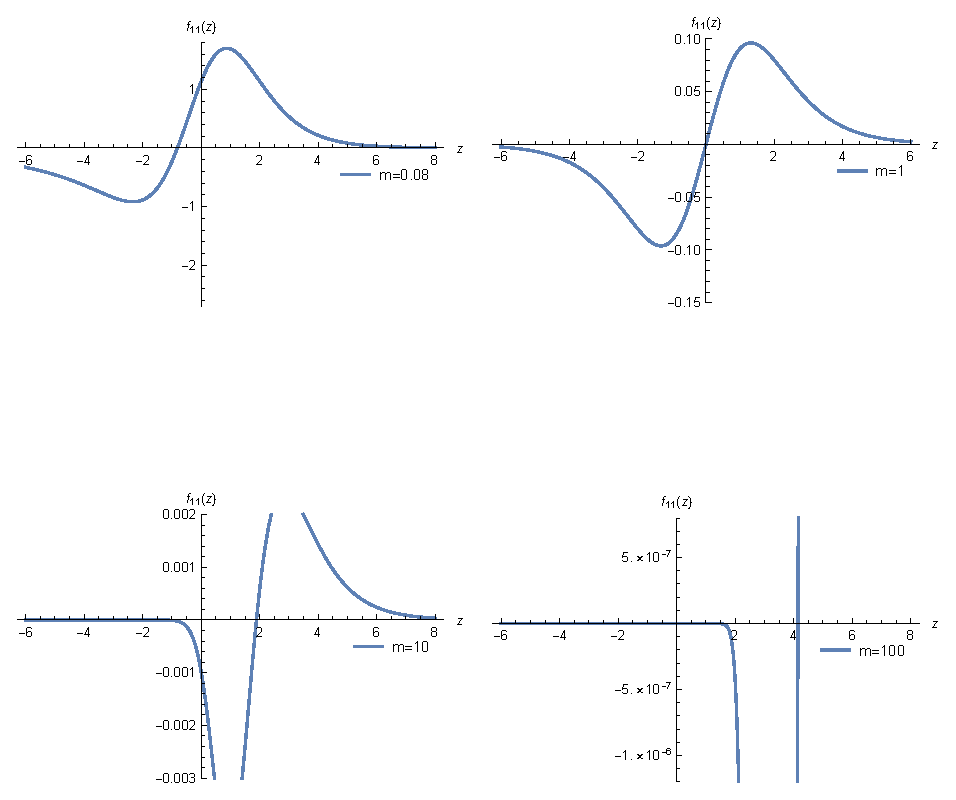
\includegraphics[scale = 0.8]{fig1.eps}
    \caption{$f_{11}(z)$ for skewed logit model, z:[-6,8], m= 0.08,1,10, and 100}
    \label{fig:skewedlogit_before}
\end{figure}


% \begin{figure}[ht]
% \subfloat[]{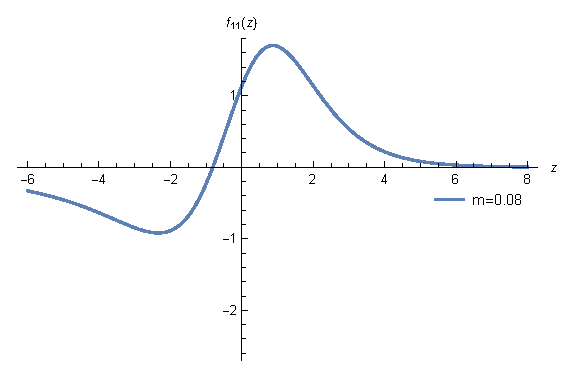
\includegraphics[width = 2.7in]{p008_before.eps}} 
% \subfloat[]{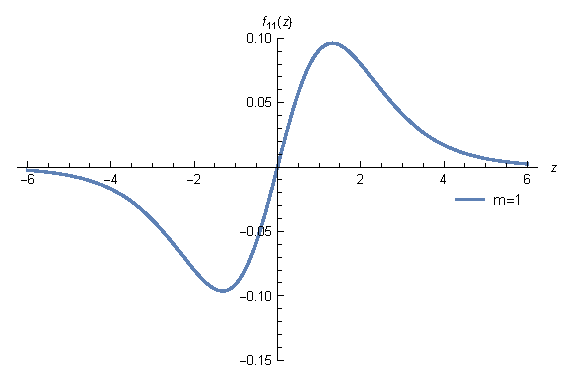
\includegraphics[width = 2.7in]{p1_before.eps}}\\
% \subfloat[]{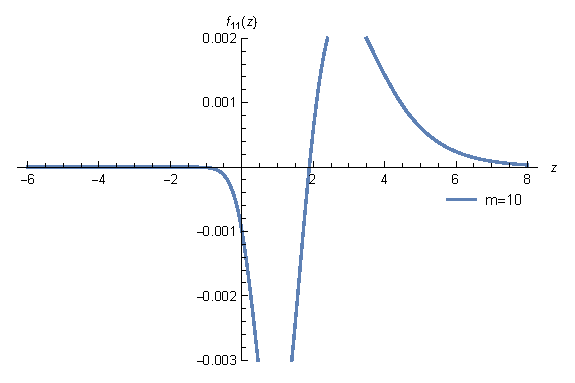
\includegraphics[width = 2.7in]{p10_before.eps}}
% \subfloat[]{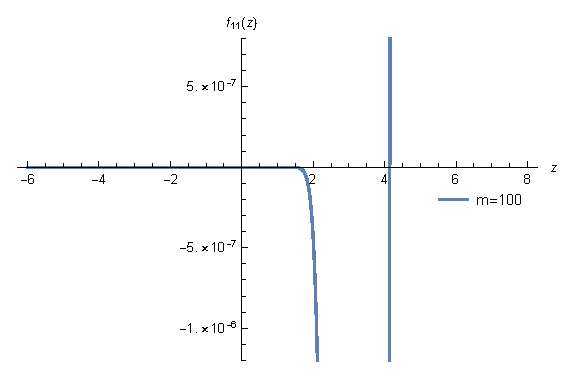
\includegraphics[width = 2.7in]{p100_before.eps}} 
% \caption{$f_{11}(z)$ for skewed logit model, z:[-6,8], m= 0.08,1,10, and 100}
% \label{fig:skewedlogit_before}
% \end{figure}
% Note that $g(z)>0$, therefore we can multiply all terms by $1/g(z)$. The sequence is now $\{1/g(z), 1,z, z^2\}$. By definition of T-system and matrix algebra, we have work instead with $\{1,z, z^2,-1/g(z)\}$. 


% We will continue with 2 of \ref{proc} and add $e^z$ to the sequence.
To resolve this issue, we insert an ancillary function $e^zg(z)$ to $S_1$, and divide all terms by $g(z)$. After proper permutation, the new sequence contains $\Psi_0(z) = 1$, $\Psi_1(z) = z$, $\Psi_2(z) = z^2$,  $\Psi_3(z) = e^z$, and $\Psi_4(z) =- (1+e^z)^2(-1+(1+e^{-z})^m)$.
Calculation shows $f_{1,1}(z) = 1$, $f_{2,2}(z) =2$, and $f_{3,3}(z) = e^z/2$. The last function $f_{4,4}(z)$ has a complicated form, and the value depends on $m$ for $z\in (-\infty, \infty)$. Specifically, numeric results show that $f_{4,4}(z)<0$ for  $z\in (-\infty, \infty)$ when $m\ge 0.2$.
\begin{figure}[ht]
    \centering
    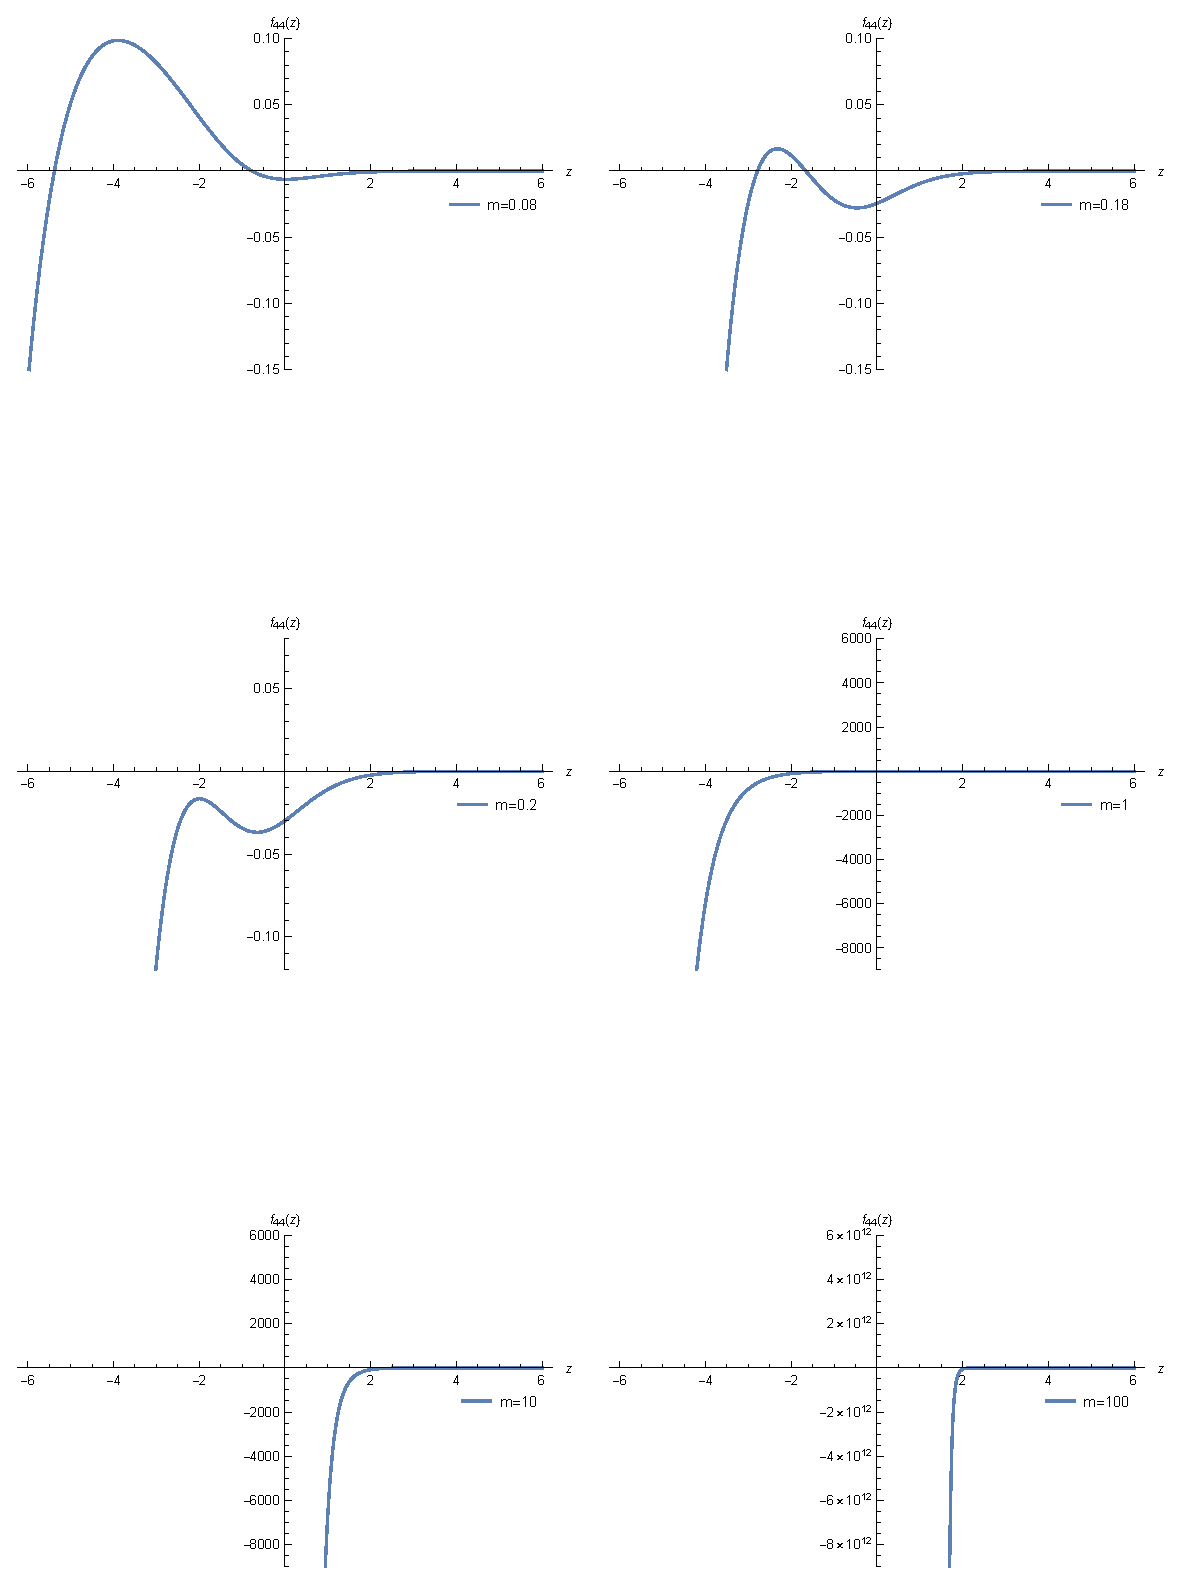
\includegraphics[scale = 0.6]{fig2.eps}
\caption{$f_{44}(z)$ for skewed logit model, z:[-6,6], m= 0.08, 0.18, 0.2,1,10, and 100}
\label{fig:skewedlogit_after}
\end{figure}

% \begin{figure}[ht]
% \subfloat[]{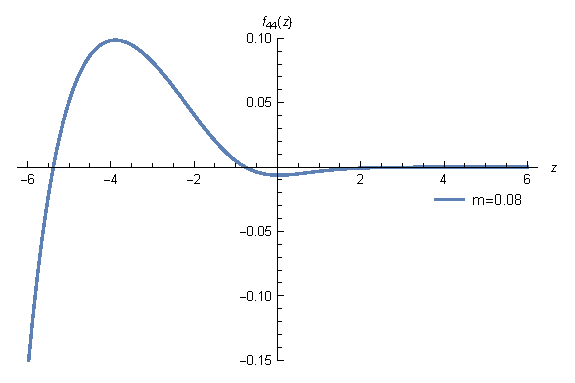
\includegraphics[width = 2.7in]{p008.eps}} 
% \subfloat[]{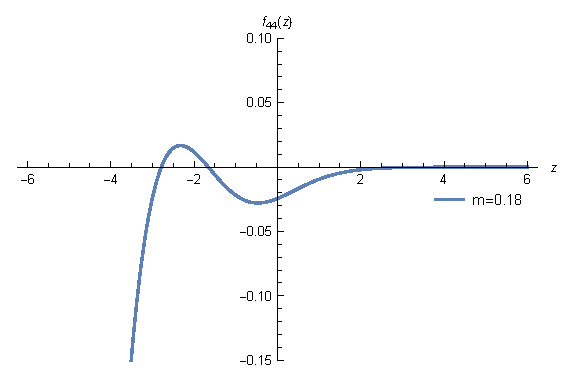
\includegraphics[width = 2.7in]{p018.eps}} \\
% \subfloat[]{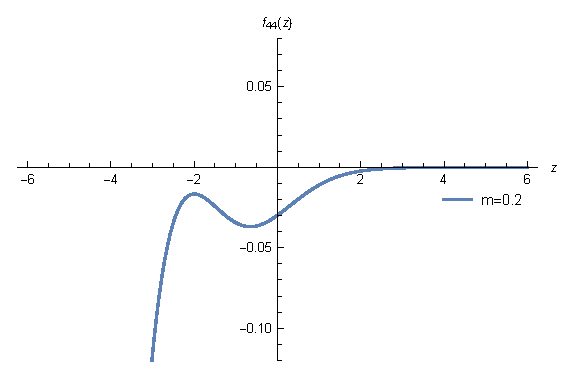
\includegraphics[width = 2.7in]{p02.eps}} 
% \subfloat[]{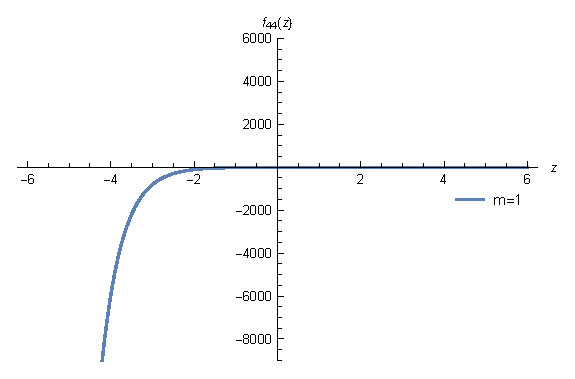
\includegraphics[width = 2.7in]{p1.eps}}\\
% \subfloat[]{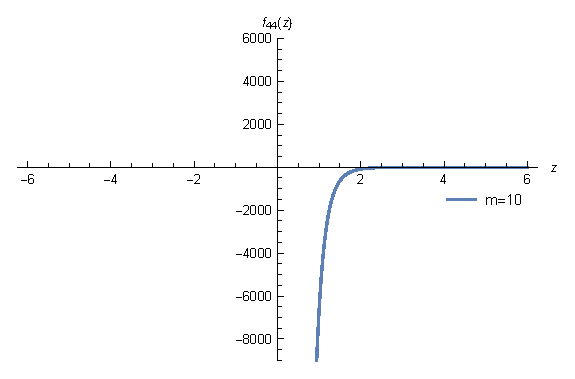
\includegraphics[width = 2.7in]{p10.eps}}
% \subfloat[]{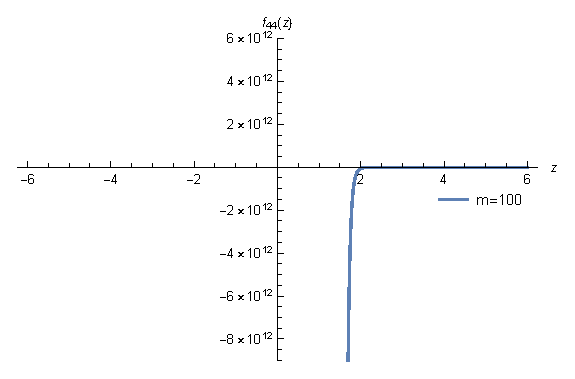
\includegraphics[width = 2.7in]{p100.eps}} 
% \caption{$f_{44}(z)$ for skewed logit model, z:[-6,6], m= 0.08, 0.18, 0.2,1,10, and 100}
% \label{fig:skewedlogit_after}
% \end{figure}
\begin{figure}[ht]
    \centering
    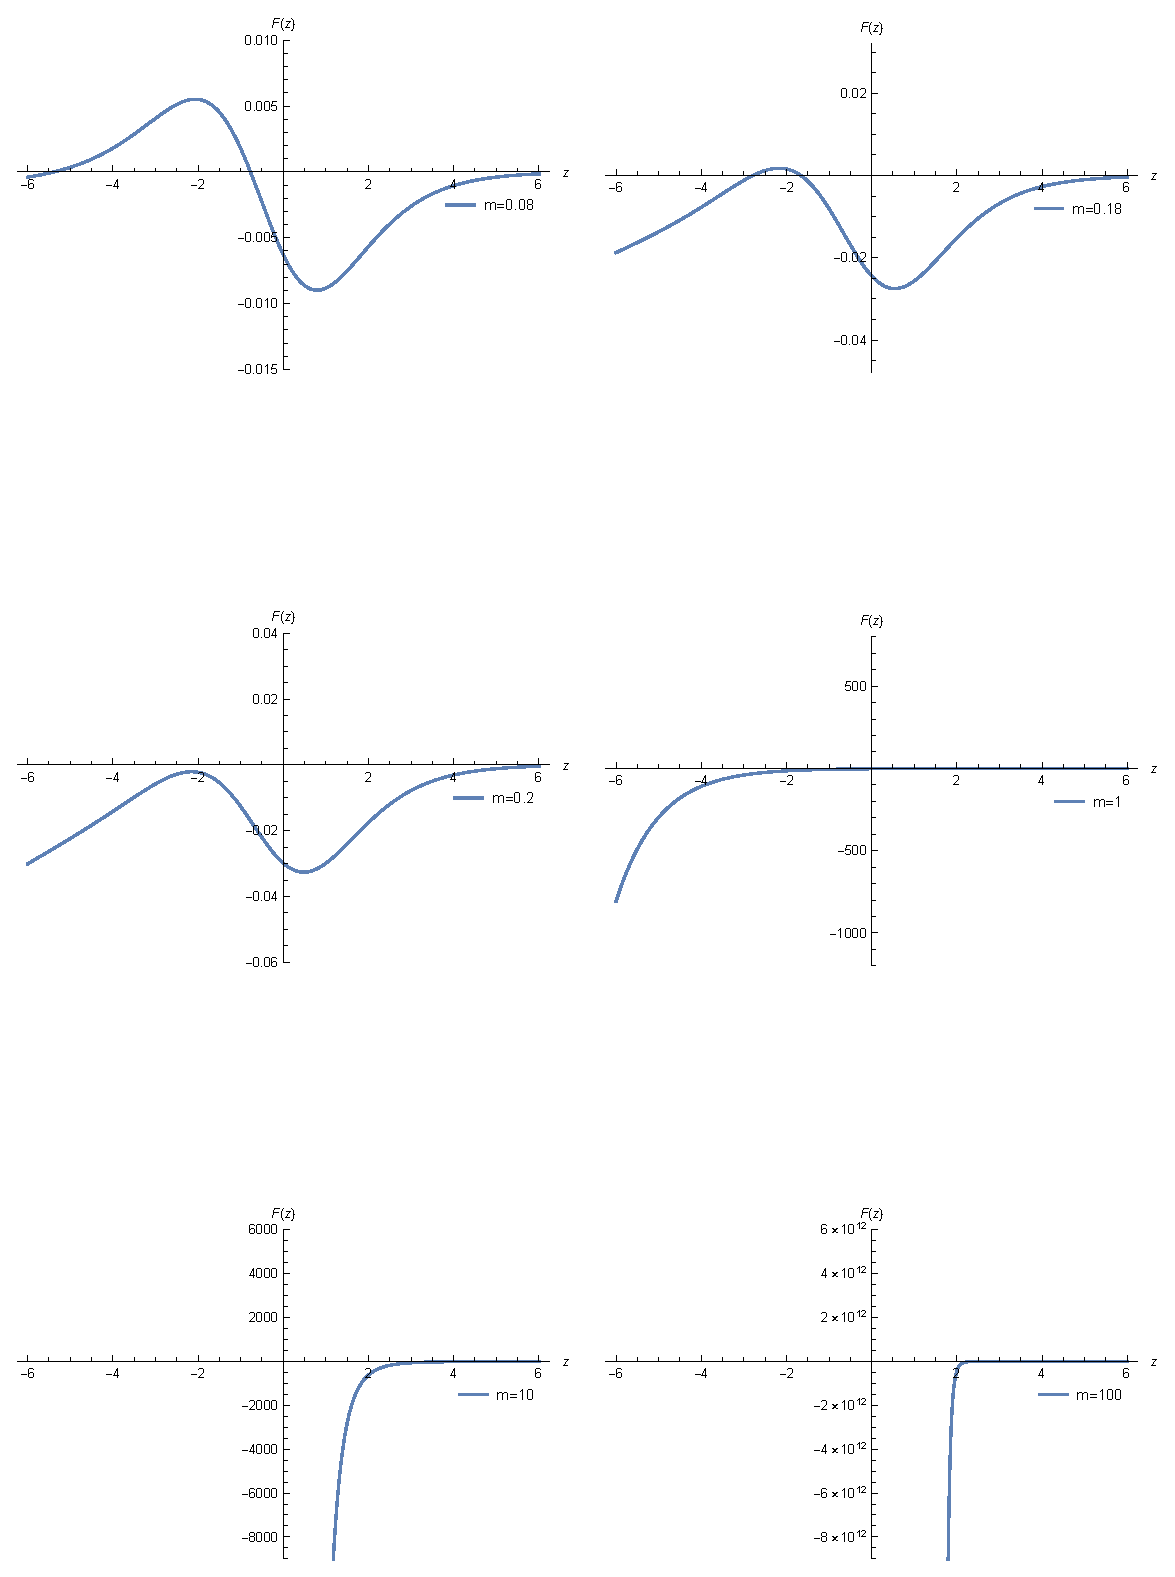
\includegraphics[scale = 0.6]{fig3.eps}
\caption{$F(z)$ for skewed logit model, z:[-6,6], m= 0.08, 0.18, 0.2,1,10, and 100}
\label{fig:skewedlogit_after_F}
\end{figure}
% \begin{figure}[ht]
% \subfloat[]{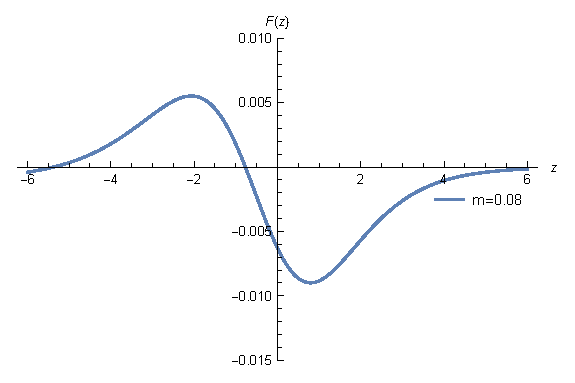
\includegraphics[width = 2.7in]{p008_F.eps}} 
% \subfloat[]{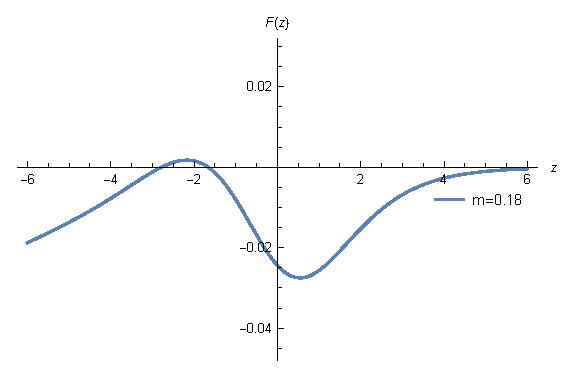
\includegraphics[width = 2.7in]{p018_F.eps}} \\
% \subfloat[]{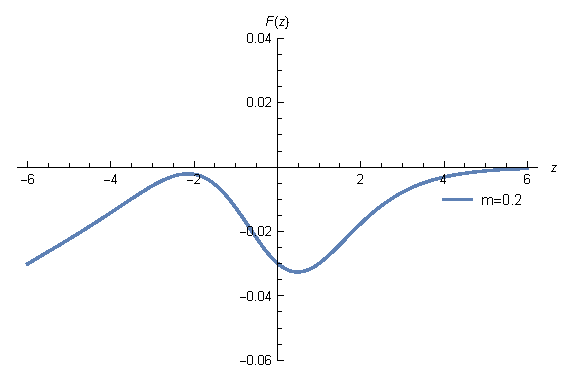
\includegraphics[width = 2.7in]{p02_F.eps}} 
% \subfloat[]{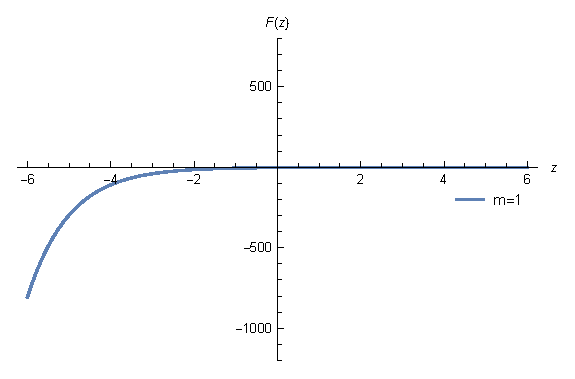
\includegraphics[width = 2.7in]{p1_F.eps}}\\
% \subfloat[]{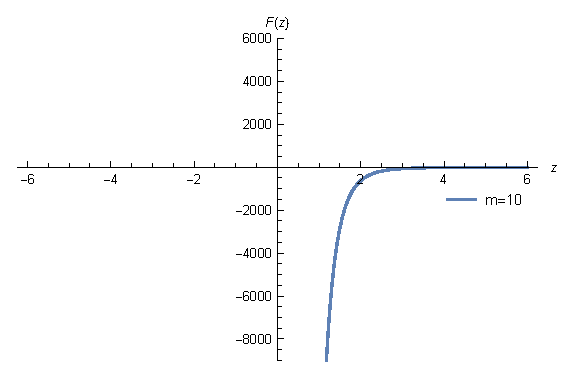
\includegraphics[width = 2.7in]{p10_F.eps}}
% \subfloat[]{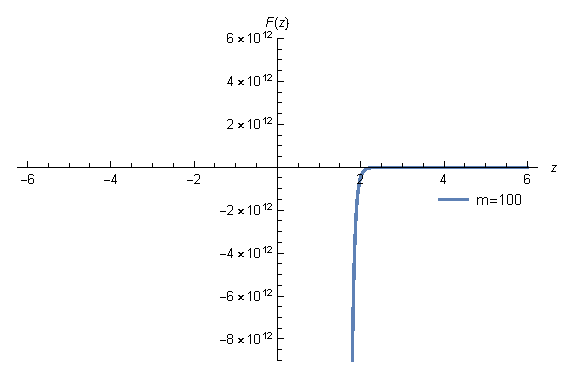
\includegraphics[width = 2.7in]{p100_F.eps}} 
% \caption{$F(z)$ for skewed logit model, z:[-6,6], m= 0.08, 0.18, 0.2,1,10, and 100}
% \label{fig:skewedlogit_after_F}
% \end{figure}
Figures~\ref{fig:skewedlogit_after}-\ref{fig:skewedlogit_after_F} demonstrate $f_{4,4}(z)$ and $F(z)$ after use of ancillary functions for $m = 0.08, 0.18,$ $ 0.2, 1, 10$, and $100$. For $m\ge0.2$, both $f_{4,4}(z)$ and $F(z)$ do not intersect the horizontal axis, which validate the assumptions.
Unfortunately, we are not able to provide analytical proof of this result. The behavior of $f_{4,4}(z)$ and $F(z)$ for $m\in(0,0.2)$ remains to be resolved with more advanced tools. 


%While we cannot analytically prove that the  $F(z)=0$ does not have solution for $z\in (-\infty,\infty)$, we plot the $F(z)$ surface with Mathematica and observe that the surface remains below $F(z)=0$ (see Figure~\ref{fig:skewedlogit_after}). As a result, with the speculation $F(z)<0$ for $z\in (-\infty,\infty)$, the assumptions are satisfied. 

As a result of this speculation, we have $F(z)<0$ for $z\in (-\infty,\infty)$ when $m\ge 0.2$, and the assumptions are satisfied. Applying results from Yang \& Stufken (2012), we know that considering $z\in[L,U]$ for any large $L<0$ and $U$, the designs with at most 3 support points including $U$ form a complete class. Further more, since this model is a Type III model with 2 parameters, through Theorem 1, there always exists a complete class of 2 support points that contains the optimal design for $m\ge0.2$. The conclusions are summarized in Conjecture 1.
% \begin{multline*}
%      -f_{4,4} = e^{-z} \left(3 (m-1) m e^{-2 z} \left(2 e^z \left(e^z+1\right)+2 e^{2 z}\right) \left(e^{-z}+1\right)^{m-2}+3 m e^{-z} \left(2 e^z \left(e^z+1\right)+2 e^{2 z}\right) \left(e^{-z}+1\right)^{m-1}-4 m e^{-z} \left(2 e^z \left(e^z+1\right)+6 e^{2 z}\right) \left(e^{-z}+1\right)^{m-1}+\left(2 e^z \left(e^z+1\right)+14 e^{2 z}\right) \left(\left(e^{-z}+1\right)^m-1\right)+6 e^{2 z} \left((m-1) m e^{-2 z} \left(e^{-z}+1\right)^{m-2}+m e^{-z} \left(e^{-z}+1\right)^{m-1}\right)+6 e^z \left(e^z+1\right) \left((m-1) m e^{-2 z} \left(e^{-z}+1\right)^{m-2}+m e^{-z} \left(e^{-z}+1\right)^{m-1}\right)+\left(e^z+1\right)^2 \left((m-3) (m-2) (m-1) m e^{-4 z} \left(e^{-z}+1\right)^{m-4}+6 (m-2) (m-1) m e^{-3 z} \left(e^{-z}+1\right)^{m-3}+7 (m-1) m e^{-2 z} \left(e^{-z}+1\right)^{m-2}+m e^{-z} \left(e^{-z}+1\right)^{m-1}\right)+8 e^z \left(e^z+1\right) \left((m-2) (m-1) m \left(-e^{-3 z}\right) \left(e^{-z}+1\right)^{m-3}-3 (m-1) m e^{-2 z} \left(e^{-z}+1\right)^{m-2}-m e^{-z} \left(e^{-z}+1\right)^{m-1}\right)\right)\\-e^{-z} \left(-3 m e^{-z} \left(2 e^z \left(e^z+1\right)+2 e^{2 z}\right) \left(e^{-z}+1\right)^{m-1}+\left(2 e^z \left(e^z+1\right)+6 e^{2 z}\right) \left(\left(e^{-z}+1\right)^m-1\right)+6 e^z \left(e^z+1\right) \left((m-1) m e^{-2 z} \left(e^{-z}+1\right)^{m-2}+m e^{-z} \left(e^{-z}+1\right)^{m-1}\right)+\left(e^z+1\right)^2 \left((m-2) (m-1) m \left(-e^{-3 z}\right) \left(e^{-z}+1\right)^{m-3}-3 (m-1) m e^{-2 z} \left(e^{-z}+1\right)^{m-2}-m e^{-z} \left(e^{-z}+1\right)^{m-1}\right)\right)
% \end{multline*}

     

\begin{theorem}{Conjecture 1}{}\label{skew}
For two parameter skewed logit model\[
P(y=1|x,\alpha,\beta) = \eta(x,\alpha,\beta)= \frac{1}{(1+e^{-\beta(x-\alpha)})^m}.
\]with a skewness parameter $m\ge0.2$, and $x\in (-\infty,+\infty)$. The designs with at most 2 points form a complete class.
\end{theorem}



Conjecture 1 provides a complete class of minimally supported designs for the two-parameter skewed logit model. This complete class contains the optimal design in terms of Loewner ordering. A similar result is provided by Biedermann, Dette, \& Zhu (2006) which used the geometric approach to show that $\Phi_p$ optimal design for skewed logit model contains two support points for $m>0$. 



\section{Discussion}\label{dis}
In this paper, we proposed a tool called ancillary functions to identify optimal designs for nonlinear models, which extends the complete class strategy in Yang (2010) and Yang \& Stufken (2012) to more nonlinear models. While the use of ancillary functions may lead to more support points in the optimal design, our result shows that added support points are asymptotically removable under certain circumstances which makes minimally supported designs available for more nonlinear models that were not feasible with previous strategies. The results facilitate a more refined and unified framework for optimal designs for nonlinear models that simplify the mathematical derivation and numerical search.

While this paper focuses on models with a single regression variable, the optimality results can potentially be generalized to models with multiple regression variables. The connection between the information matrices from the two cases helps in finding a complete class under a multiple regression model. For example, Yang, Zhang, \& Huang (2011) studied optimal designs for the logistic regression model with multiple regression variables. The results were based on the results of two parameters logistic models by Yang \& Stufken (2009) in which the foundation of complete class approach was built. How to derive the results for general nonlinear models with multiple regression variables, however, is beyond the scope of this paper.

The identification of minimally supported designs can be beneficial in many aspects. Pukelsheim \& Torsney (1991) show that closed-form solutions for designs are available when the number of support points equals the number of parameters ($n=p$), indicating that the numerical computation time can be largely scaled down for minimally supported designs.  Additionally, the resulting minimally supported design could be favorable in certain scenarios. For example, in the manufacturing industry, fewer support points in experimental design indicate fewer product prototypes, which induce less experimental cost since the production of a new prototype is often much more expensive than a replicate of an existing prototype. In the big data scenario when direct model fitting is infeasible, this framework could help identify the most informative subset for efficient parameter estimation.


There are a few topics that we did not address adequately. In the three models explored - the Beta-Poisson model, complementary log-log model, and skewed logit model - we selected some shared factors of the $\Psi(z)$ functions in the sequence as the ancillary functions, yet we didn't give a general guide on how to make the selection. The scheme of the selection remains to be discussed in future work. Additionally in Section~\ref{secskew}, due to the complexity of the skewed logit model, we did not provide a theoretical proof of $F(z)<0$ but instead used a numerical check through Mathematica for $m>0.2$. Interested readers could explore the analytical proof of Conjecture 1. More advanced tools are also called for to investigate the behavior of skewed logit model for $m\in (0,0.2)$. Last but not least, our strategy and conclusions in this paper currently only apply for information-based criteria. 


 




% \begin{ack}{ACKNOWLEDGEMENTS}
% The authors are grateful for the comments from two referees, an associate editor, and editor, which helped to improve the article. Yang’s research was supported by NSF grant DMS-1811291.
% \end{ack}
% \bibliographystyle{Cjsref}
% \bibliography{bib_t} 

\begin{thebibliography}{}
% For English spelling, we follow the style of this dictionary
\bibitem[]{bib1}
Biedermann, S., Dette, H., \& Zhu, W. (2006). Optimal designs for dose-response models with restricted design spaces. {\it Journal of the American Statistical Association}, 101(474), 747--759.
\bibitem[]{bib2}
Demidenko, Eugene (2006). The assessment of tumour response to treatment..{\it Journal of the Royal Statistical Society: Series C (Applied Statistics)}, 55(3),365-377.

\bibitem[]{bib3}
Dette, H. \& Melas, V.B. (2011). A note on the de la Garza phenomenon for locally optimal designs. {\it Annals of Statistics}, 39(2), 1266--1281.

\bibitem[]{bib4}
Dette, H.,Melas, V.B. (2011). \& Shpilev, P. (2013). Robust t-optimal discriminating designs. {\it Annals of Statistics}, 41(4), 1693--1715.

\bibitem[]{bib5}
Dette, H.,Melas, V.B. (2011). \& Wong, W. K. (2006). Locally d-optimal designs for exponential regression models. {\it Statistical Sinica}, 16(3), 789--803.

\bibitem[]{bib6}
Elfving, G. (1952). Optimum allocation in linear regression theory. {\it Annals of Statistics}, 23(2), 255--263.

\bibitem[]{bib51}
Gaudard, M. A., Karson, M. J., Linder, E., \& Tse, S. K. (1993). Efficient designs for estimation in the power logistic quantal response model. {\it Statistica Sinica}, 3, 233--243


\bibitem[]{bib7}
Haas, C. (1983). Estimation of risk due to low doses of microorganisms: A comparison of alternative methodologies. {\it American journal of epidemiology}, 118(4), 573--82.

\bibitem[]{bib62}
Hedayat, A. S., Yan, B., \& Pezzuto, J. M. (1997). Modeling and identifying optimum designs for fitting dose-response curves based on raw optical density data. {\it Journal of the American Statistical Association}, 92(439), 1132–1140.

\bibitem[]{bib71}
Karlin, S. \& Studden, W. J. (1966).  {\it Tchebycheff systems with applications in analysis and statistics}, Interscience Publishers, New York.

\bibitem[]{bib8}
Kiefer, J. \& Wolfowitz, J. (1960). Equivalence of two extremal problems. {\it Canadian Journal of Mathematics}, 14, 849--879.

\bibitem[]{bib81}
Nagler, J. (1994). Scobit: An alternative estimator to logit and probit. {\it American Journal of Political Science}, 38(1), 230–255.

\bibitem[]{bib82}
Prentice, R. L. (1976). A generalization of the probit and logit methods for dose response curves. {\it Biometrics}, 32(4), 761–768.

\bibitem[]{bib83}
Pukelsheim, F. \& Torsney, B. (1991) Optimal weights for experimental designs on linearly independent support points, {\it Annals of Statistics}, 19, 1614--1625.



\bibitem[]{bib9}
Ruzante, J., Whiting, R., Dennis, S., \& Buchanan, R. (2013). {\it Microbial Risk Assessment}, ASM Press.

\bibitem[]{bib10}
Wang, H., Yang, M., \& Stufken, J. (2018). Information-based optimal subdata selection for big data linear regression. {\it Journal of the American Statistical Association}, 114(525), 393--405.

\bibitem[]{bib11}
Yang, M. (2010). On the de la garza phenomenon. {\it Annals of Statistics}, 38(4), 2499--2524.

\bibitem[]{bib12}
Yang, M. \& Stufken, J. (2009). Support points of locally optimal designs for nonlinear models with two parameters. {\it Annals of Statistics}, 37(1), 518--541.

\bibitem[]{bib13}
Yang, M. \& Stufken, J. (2012). Identifying locally optimal designs for nonlinear models: A simple extension with profound consequences. {\it Annals of Statistics}, 40(3), 1665--1681.
\bibitem[]{bib131}
Yang, M., Zhang, B. \& Huang, S. (2011). Optimal designs for generalized linear models with multiple design variables. {\it Statistica Sinica}, 21, 1415--1430

\bibitem[]{bib14}
Zhai, Y. \& Fang, Z. (2018). Locally optimal designs for binary dose-response models. {\it Canadian Journal of Statistics}, 46(2), 336--354.












\end{thebibliography}




% \begin{appendix}
% There should be just one appendix, for proofs and longer
% mathematical arguments. These proofs are in the following form:

% \begin{proof}{Proof of Theorem 1}{}%
% We now prove the two parts of Theorem 1.
% \end{proof}
% \end{appendix}

\CJShistory
\end{document}
